\documentclass[12pt]{article}

\usepackage[utf8]{inputenc}
\usepackage{graphicx}
\usepackage{latexsym,amsfonts,amssymb,amsthm,amsmath}
\usepackage{tikz}
\usepackage{listings}
\usepackage[left=1 in, right=0.5in, top=0.5in, bottom=0.5in]{geometry}

\usepackage{enumitem} % For better list formatting
\usepackage{bm}       % Required for bold math symbols (\bm)   % Required for drawing flowcharts
\usetikzlibrary{shapes.geometric, arrows, calc, patterns}



\usepackage{xcolor} % For color options

% Define custom colors for the code
\definecolor{mymauve}{rgb}{0.58, 0.0, 0.83}
\definecolor{mygreen}{rgb}{0.0, 0.5, 0.0}
\definecolor{mygray}{rgb}{0.5, 0.5, 0.5}


% Set up the listings package
\lstset{
    language=Matlab,                % Set language to Matlab
    basicstyle=\ttfamily\small,     % Use monospaced font
    keywordstyle=\color{blue},      % Color keywords blue
    stringstyle=\color{purple},     % Color strings purple
    commentstyle=\color{green!50!black}, % Color comments green
    showstringspaces=false,         % <--- CRITICAL: Hides the visible space marker in strings
    breaklines=true,                % Wrap long lines
    numbers=left,                   % Line numbers on left
    numberstyle=\tiny\color{gray},  % Line number style
    frame=single,                   % Box around code
    backgroundcolor=\color{gray!5}  % Light gray background
}



\title{ME 5310 -  Finite Element Project }
\author{\textbf{Name: Shuvo Chowdhury} \\ Student ID: 1002238403}
\date{}  % This removes the date

\begin{document}

\maketitle

\vspace{-0.5in}

\section*{\textbf{2D FE Code}}
\subsection*{Algorithm}
The finite element code is organized into four modular files to separate the global logic from the element-level mathematics.

\begin{enumerate}
    \item \textbf{Main\_Project.m (Driver Script):} This is the primary execution file. It handles input definitions, mesh generation, the global assembly loop, boundary condition applications, the linear solver, and output plotting.
    \item \textbf{Quad4Stiffness.m (Function):} A helper function called during the assembly phase. It accepts element coordinates and material properties, performs Gaussian quadrature, and returns the $8 \times 8$ element stiffness matrix ($\mathbf{k}^e$).
    \item \textbf{CalcStress.m (Function):} A helper function called during post-processing. It accepts deformed element coordinates and nodal displacements to calculate the stress tensor ($\bm{\sigma}$) and Von Mises stress.
        \item \textbf{PlotMesh.m (Function):} A helper function to plot the deformed and undeformed configuration of the mesh.
\end{enumerate}

\begin{figure}[h]
\centering
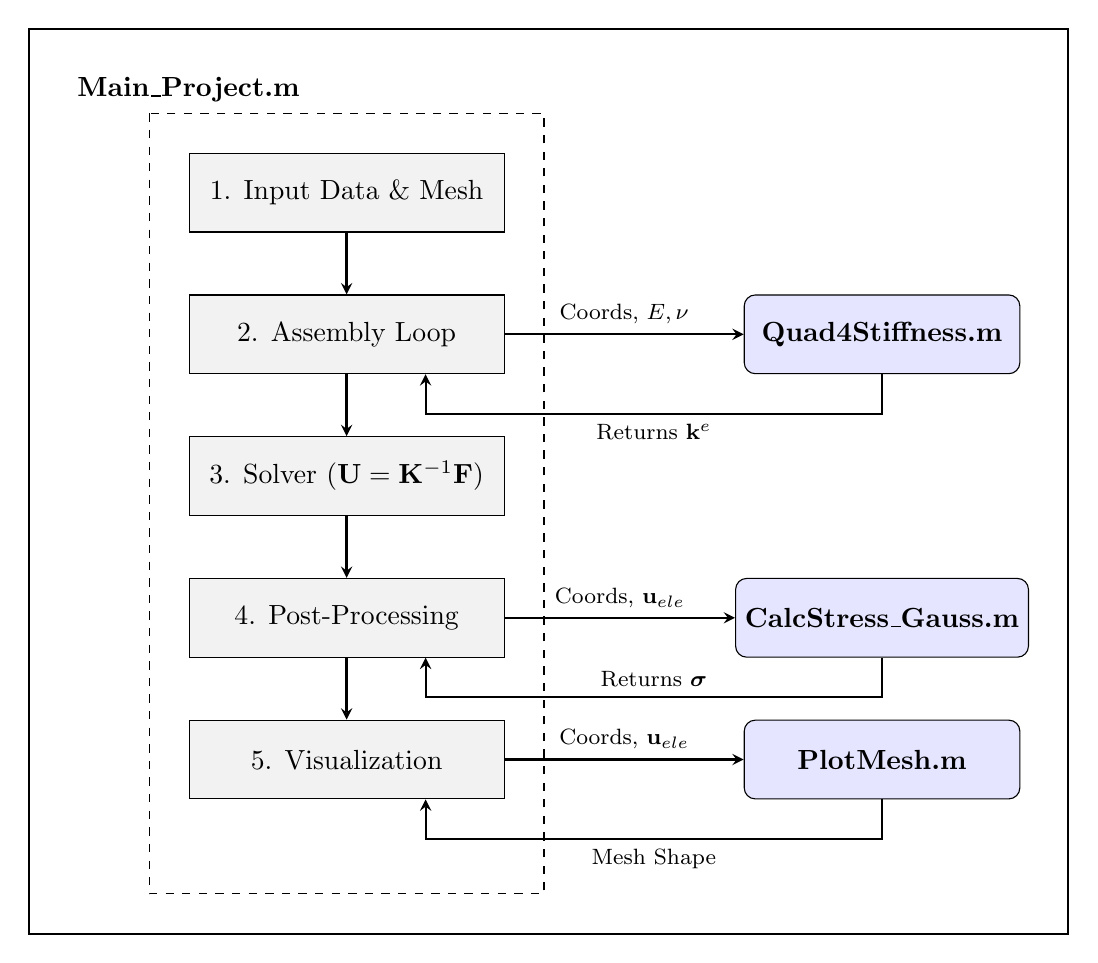
\begin{tikzpicture}[node distance=1.8cm]
\tikzstyle{main} = [rectangle, minimum width=4cm, minimum height=1cm, text centered, draw=black, fill=gray!10]
\tikzstyle{func} = [rectangle, minimum width=3.5cm, minimum height=1cm, text centered, draw=black, fill=blue!10, rounded corners]
\tikzstyle{arrow} = [thick,->,>=stealth]

% Main Script Nodes
\node (input) [main] {1. Input Data \& Mesh};
\node (loop) [main, below of=input] {2. Assembly Loop};
\node (solve) [main, below of=loop] {3. Solver ($\mathbf{U} = \mathbf{K}^{-1}\mathbf{F}$)};
\node (post) [main, below of=solve] {4. Post-Processing};
\node (vis) [main, below of=post] {5. Visualization};

% Function Nodes
\node (stiff) [func, right of=loop, xshift=5cm] {\textbf{Quad4Stiffness.m}};
\node (calc) [func, right of=post, xshift=5cm] {\textbf{CalcStress\_Gauss.m}};
\node (plot) [func, right of=vis, xshift= 5cm] {\textbf{PlotMesh.m}};

% Main Flow Arrows
\draw [arrow] (input) -- (loop);
\draw [arrow] (loop) -- (solve);
\draw [arrow] (solve) -- (post);
\draw [arrow] (post) -- (vis);

% Interaction Arrows (Stiffness)
\draw [arrow] (loop.east) -- node[above, font=\footnotesize] {Coords, $E, \nu$} (stiff.west);
\draw [arrow] (stiff.south) -- ++(0,-0.5) -| node[near start, below, font=\footnotesize] {Returns $\mathbf{k}^e$} ($(loop.south east)!0.5!(loop.south)$);

% Interaction Arrows (Stress)
\draw [arrow] (post.east) -- node[above, font=\footnotesize] {Coords, $\mathbf{u}_{ele}$} (calc.west);
\draw [arrow] (calc.south) -- ++(0,-0.5) -| node[near start, above, font=\footnotesize] {Returns $\bm{\sigma}$} ($(post.south east)!0.5!(post.south)$);

% Interaction Arrows (Visualization)
\draw [arrow] (vis.east) -- node[above, font=\footnotesize] {Coords, $\mathbf{u}_{ele}$} (plot.west);
\draw [arrow] (plot.south) -- ++(0,-0.5) -| node[near start, below, font=\footnotesize] {Mesh Shape} ($(vis.south east)!0.5!(vis.south)$);


% Dashed Box for Main Script
\draw[dashed] ($(input.north west)+(-0.5,0.5)$) rectangle ($(vis.south east)+(0.5,-1.2)$);
\node at ($(input.north west)+(0,0.8)$) {\textbf{Main\_Project.m}};

% --- Bounding Box for Entire Figure ---
% Calculates a rectangle based on the current bounding box of all drawn elements plus some padding
\draw[thick, black] ($(current bounding box.north west)+(-0.5,0.5)$) rectangle ($(current bounding box.south east)+(0.5,-0.5)$);


\end{tikzpicture}
\caption{Data flow diagram showing the interaction between the main driver script and the helper functions.}
\end{figure}

\subsection*{Step 1: Initialization and Input}
\begin{enumerate}
    \item Define material properties: Young's Modulus ($E$), Poisson's Ratio ($\nu$), and thickness ($t$).
    \item Define the mesh:
    \begin{itemize}
        \item Load the \textbf{Nodes} list (coordinates $x, y$).
        \item Load the \textbf{Elements} connectivity list (node IDs for each element).
    \end{itemize}
    \item Initialize the global stiffness matrix $\mathbf{K}$ (size $2N \times 2N$) with zeros.
    \item Initialize the global force vector $\mathbf{F}$ (size $2N \times 1$) with zeros.
    \item Calculate the material constitutive matrix $\mathbf{D}$ for Plane Stress conditions.
\end{enumerate}

\subsection*{Step 2: Stiffness Matrix Assembly}
Loop over every element in the mesh:
\begin{enumerate}
    \item Extract the coordinates of the 4 nodes belonging to the current element.
    \item Initialize the element stiffness matrix $\mathbf{k}^e$ (size $8 \times 8$).
    \item \textbf{Numerical Integration (Gaussian Quadrature):}
    \begin{enumerate}
        \item Loop through the 4 Gauss points ($\xi = \pm 0.577, \eta = \pm 0.577$).
        \item Calculate derivatives of shape functions with respect to natural coordinates ($\xi, \eta$).
        \item Compute the Jacobian matrix $\mathbf{J}$ and its determinant $|\mathbf{J}|$.
        \item Transform derivatives to physical coordinates ($x, y$) using $\mathbf{J}^{-1}$.
        \item Construct the strain-displacement matrix $\mathbf{B}$.
        \item Compute the local stiffness contribution: $\mathbf{B}^T \mathbf{D} \mathbf{B} \cdot |\mathbf{J}| \cdot \text{weight} \cdot \text{thickness}$.
        \item Add this contribution to $\mathbf{k}^e$.
    \end{enumerate}
    \item \textbf{Assembly:} Map the local indices of $\mathbf{k}^e$ to the global indices in $\mathbf{K}$ and add the values.
\end{enumerate}

\subsection*{Step 3: Boundary Conditions and Loading}
\begin{enumerate}
    \item Apply external forces to the global force vector $\mathbf{F}$ at the specified node degrees of freedom (DOFs).
    \item Identify the list of \textbf{Fixed DOFs} (where displacement is constrained to 0).
    \item Identify the list of \textbf{Free DOFs} (the unknowns we need to solve for).
\end{enumerate}

\subsection*{Step 4: Solution}
\begin{enumerate}
    \item Extract the sub-matrix $\mathbf{K}_{free}$ containing only the rows/columns of Free DOFs.
    \item Extract the sub-vector $\mathbf{F}_{free}$ containing only the forces at Free DOFs.
    \item Solve the linear system of equations: 
    \[ \mathbf{K}_{free} \cdot \mathbf{U}_{free} = \mathbf{F}_{free} \]
    \item Reconstruct the full displacement vector $\mathbf{U}$ by filling Fixed DOFs with zeros.
\end{enumerate}

\subsection*{Step 5: Post-Processing (Stress Calculation)}
Loop over every element again:
\begin{enumerate}
    \item Extract the computed displacements for the element's nodes.
    \item Calculate the $\mathbf{B}$ matrix at the element centroid (or integration points).
    \item Compute Strain: $\bm{\epsilon} = \mathbf{B} \cdot \mathbf{u}_{element}$.
    \item Compute Stress: $\bm{\sigma} = \mathbf{D} \cdot \bm{\epsilon}$.
    \item Calculate Von Mises stress for yield criteria checking.
\end{enumerate}
\newpage

\subsection*{\textbf{Matlab Code}}
\subsubsection*{Main\_Project.m}
\begin{lstlisting}[language=Matlab]
% ==========================================
% ME 5310 -  Finite Element Project
% 2D Plane Stress Elasticity Solver
% File: Main_Project.m (Driver Script)
% ==========================================
clc; clear; close all;
%% 1. Input Data (Set up for test case A: Single Element Validation)
%-------------------------------------------
% Material Properties
E  = 30e6;
nu = 0.3;
t = 1; %Thickness

% Mesh Definition
% Nodes List: [Node ID, x-coord, y-coord]
Nodes = [
  1, 0.0, 0.0;
  2, 1.0, 0.0;
  3, 1.0, 1.0;
  4, 0.0, 1.0
    ];

% Element Connectivity: [Elem ID, Node 1, Node 2, Node 3, Node 4]
% Note: Nodes must be listed in counter-clockwise order.
Elements = [
    1,   1,   2,  3,  4; 
];

% Problem Size Parameters
num_nodes = size(Nodes, 1);
num_elems = size(Elements, 1);
num_dofs = num_nodes * 2; % 2 DOFs per node (u, v)

%% 2. INITIALIZATION
% ------------------------------------------------
% Initialize global stiffness matrix (Sparse is better for large problems)
K_global = sparse(num_dofs, num_dofs);
F_global = zeros(num_dofs, 1);
U_global = zeros(num_dofs, 1);

%% 3. ASSEMBLY PROCESS
% -------------------------------------------------
disp('Assembling Global Stiffness Matrix...');

for e = 1: num_elems
    % A. extract node IDs for this element 
    node_ids = Elements(e, 2:5);

    % B. Extract coordinates for this node
    ele_coords = Nodes(node_ids, 2:3);

    % C. Compute element stiffness matrix
    k_e = Quad4Stiffness (ele_coords, E, nu, t);

    % D. Mapping to the global matrix by a scatter vector

    scatter = zeros (1,8);

    for n = 1:4
        global_node= node_ids(n);
        scatter(2*n-1) = 2*global_node - 1; % x-dof (Odd index)
        scatter(2*n)   = 2*global_node;     % y-dof (Even index)
    end

    % E. Add to global matrix
    K_global(scatter, scatter) = K_global(scatter, scatter) + k_e;

end


%% 4. APPLY BOUNDARY CONDITIONS (BCs) & LOADS
% ----------------------------------------

fixed_nodes_u = [1, 4]; % Nodes fixed in X
fixed_nodes_v = [1, 4]; % Nodes fixed in Y

% Convert Node IDs to DOF Indices
fixed_dofs = [ (2*fixed_nodes_u - 1), (2*fixed_nodes_v) ]; % [1, 2, 4, 7]
fixed_dofs = unique(fixed_dofs); % Remove duplicates % [1, 2, 4, 7]

% Free DOFs are all other DOFs
all_dofs = 1:num_dofs;  % [1, 2, 3, 4, 5, 6,7,8]
free_dofs = setdiff(all_dofs, fixed_dofs);   % [3, 5, 6,8]

% B. Apply External Forces (Point Loads)
% Test Case Setup: Apply Tension in Y-direction at top nodes (3 & 4)
% Load P = 1000 lbs split between top nodes.
P_load = 100; 
load_nodes = [2,3];


for i = 1:length(load_nodes)
    node = load_nodes(i);
    dof_y = 2*node-1; % y-dof
    F_global(dof_y) = F_global(dof_y) + P_load;
end

%% 5. SOLVER
% ---------------------------------------
disp('Solving system equations...');

% Partition the system (Extract only free DOFs)
K_ff = K_global(free_dofs, free_dofs);
F_f  = F_global(free_dofs);

% Solve for unknown displacements [cite: 65]
U_f = K_ff \ F_f;

% Reconstruct the full displacement vector
U_global(free_dofs) = U_f;
U_global(fixed_dofs) = 0; % Enforce zero at fixed supports

disp('Nodal Displacements:');
disp(U_global);

% %% 6. POST-PROCESSING
% % ------------------------------------
disp('Calculating Element Stresses at Integration Points...');

for e = 1:num_elems
    node_ids = Elements(e, 2:5);
    ele_coords = Nodes(node_ids, 2:3);

    % Extract displacements
    u_ele = zeros(8,1);
    for n = 1:4
        global_node = node_ids(n);
        u_ele(2*n-1) = U_global(2*global_node - 1);
        u_ele(2*n)   = U_global(2*global_node);
    end

    % Calculate Stress at 4 Gauss Points
    [stress_mat, vm_vec] = CalcStress_Gauss(ele_coords, u_ele, E, nu);

    % Print Results
    fprintf('\nElement %d Results:\n', e);
    fprintf('  GP | Sig_xx   | Sig_yy   | Tau_xy   | VonMises\n');
    fprintf('  ---|----------|----------|----------|---------\n');
    for gp = 1:4
        fprintf('  %d  | %8.2f | %8.2f | %8.2f | %8.2f\n', ...
            gp, stress_mat(gp,1), stress_mat(gp,2), stress_mat(gp,3), vm_vec(gp));
    end
end

disp('Analysis Complete.');
disp('Plotting input mesh...');
PlotMesh(Nodes, Elements);

disp('Plotting deformed shape...');
% scale = 1000; % Exaggerate deformation to make it visible
% PlotMesh(Nodes, Elements, U_global, 1);
disp('Plotting Superimposed shape')

figure;
hold on;
% 1. Plot undeformed mesh
PlotMesh(Nodes, Elements);
scale = 10000; % Exaggerate deformation to make it visible
PlotMesh(Nodes, Elements, U_global, scale);

%title(['Superimposed Deformation (Scale: ', num2str(scale), ')']);
axis equal;
grid on;
hold off;    % Release the hold

\end{lstlisting}

\subsubsection*{Quad4Stiffness.m}

\begin{lstlisting}[language=Matlab]
% ========================================
%  Function: Quad4Stiffness
%  Purpose:  Calculates the 8x8 Element Stiffness Matrix for a 
%            4-Node Isoparametric Quadrilateral in Plane Stress.
%
%  Inputs:
%    coords - 4x2 matrix of node coordinates [x1 y1; x2 y2; x3 y3; x4 y4]
%    E      - Young's Modulus
%    nu     - Poisson's Ratio
%    t      - Thickness
%
%  Outputs:
%    ke     - 8x8 Element Stiffness Matrix
% =========================================

function [ke] = Quad4Stiffness(coords, E, nu, t)

    % 1. CONSTITUTIVE MATRIX (D) - Plane Stress Setup
    C = E/(1-nu^2);
    D = C* [1 nu 0;
            nu 1 0;
            0 0 (1-nu)/2];
    pt = 1 / sqrt(3);           % Location of points +/- 0.57735
    w  = 1.0;                   % Weight is 1.0 for all points in 2x2 rule

    % Gauss points (xi, eta)
    GP_xi  = [-pt,  pt,  pt, -pt];
    GP_eta = [-pt, -pt,  pt,  pt];

    % Initialize Element Stiffness Matrix
    ke = zeros(8, 8);
    
    % 3. Integration points

    for i = 1:4
        xi = GP_xi(i);
        eta = GP_eta(i);

        % N1 = 0.25*(1-xi)*(1-eta)
        % N2 = 0.25*(1+xi)*(1-eta)
        % N3 = 0.25*(1+xi)*(1+eta)
        % N4 = 0.25*(1-xi)*(1+eta)

        % dN_dxi (1x4 vector)
        dN_dxi  = 0.25 * [ -(1-eta),  (1-eta),  (1+eta), -(1+eta) ];
        
        % dN_deta (1x4 vector)
        dN_deta = 0.25 * [ -(1-xi),  -(1+xi),   (1+xi),   (1-xi)  ];

        % B. JACOBIAN MATRIX (J)
        % J = [ dx/dxi   dy/dxi ]
        %     [ dx/deta  dy/deta]
        % computed as (dN_dnatural * coords)
        
        J = [dN_dxi; dN_deta] * coords;

        detJ = det(J); % Determinant of Jacobian (Area scaling factor)
        
        % Check for distorted elements (Area must be positive)
        if detJ <= 0
            error('Element Jacobian is non-positive. Check node numbering (Counter-Clockwise).');
        end

        % C. DERIVATIVES wrt PHYSICAL COORDS (x, y)
        % [dN_dx] = inv(J) * [dN_dxi ]
        % [dN_dy]            [dN_deta]
        
        %invJ = inv(J);
        dN_dxy = J\ [dN_dxi; dN_deta]; % invJ * [dN_dxi; dN_deta]; % 2x4 Matrix
        
        dN_dx = dN_dxy(1, :); % Top row is dN/dx
        dN_dy = dN_dxy(2, :); % Bottom row is dN/dy

        % D. ASSEMBLE B-MATRIX (Strain-Displacement Matrix) [cite: 62]
        % B is 3x8. Each node "j" fills 2 columns.
        % Format:
        % [ N1,x   0     N2,x   0     ... ]
        % [ 0      N1,y  0      N2,y  ... ]
        % [ N1,y   N1,x  N2,y   N2,x  ..

        B = zeros(3, 8);
        for n = 1:4
            col_u = 2*n - 1; % Column for u-displacement
            col_v = 2*n;     % Column for v-displacement
            
            B(1, col_u) = dN_dx(n);
            B(1, col_v) = 0;
            
            B(2, col_u) = 0;
            B(2, col_v) = dN_dy(n);
            
            B(3, col_u) = dN_dy(n);
            B(3, col_v) = dN_dx(n);
        end

        % E. STIFFNESS ACCUMULATION
        % ke = Sum ( B' * D * B * detJ * weight * thickness )
        ke = ke + (B' * D * B) * detJ * w * w * t;
    end
end

    

\end{lstlisting}

\subsubsection*{CalStress\_Gauss.m}

\begin{lstlisting}[language=Matlab]
function [stress_matrix, vm_vec] = CalcStress_Gauss(coords, u_ele, E, nu)
% ==============================================
%  Function: CalcStress_Gauss
%  Purpose:  Calculates stress at ALL 4 Integration Points (Gauss Points)
%
%  Inputs:
%    coords - 4x2 matrix of node coordinates
%    u_ele  - 8x1 vector of element displacements
%    E, nu  - Material properties
%
%  Outputs:
%    stress_matrix - 4x3 matrix containing stress at each Gauss point.
%                    Rows: Gauss Point 1 to 4
%                    Cols: [Sig_xx, Sig_yy, Tau_xy]
%    vm_vec        - 4x1 vector of Von Mises stress at each Gauss point
% ================================================

    % 1. CONSTITUTIVE MATRIX (D)
    C = E / (1 - nu^2);
    D = C * [ 1   nu  0 ;
              nu  1   0 ;
              0   0   (1-nu)/2 ];

    % 2. GAUSS POINTS (Same as Stiffness Matrix)
    pt = 1 / sqrt(3); 
    GP_xi  = [-pt,  pt,  pt, -pt];
    GP_eta = [-pt, -pt,  pt,  pt];
    
    % Initialize Outputs
    stress_matrix = zeros(4, 3);
    vm_vec = zeros(4, 1);

    % 3. LOOP OVER GAUSS POINTS
    for i = 1:4
        xi  = GP_xi(i);
        eta = GP_eta(i);
        
        % A. Derivatives at this Gauss Point
        dN_dxi  = 0.25 * [ -(1-eta),  (1-eta),  (1+eta), -(1+eta) ];
        dN_deta = 0.25 * [ -(1-xi),  -(1+xi),   (1+xi),   (1-xi)  ];
        
        % B. Jacobian
        J = [dN_dxi; dN_deta] * coords;
        invJ = inv(J);
        
        % C. Global Derivatives
        dN_dxy = invJ * [dN_dxi; dN_deta];
        dN_dx = dN_dxy(1, :);
        dN_dy = dN_dxy(2, :);
        
        % D. B-Matrix Construction
        B = zeros(3, 8);
        for n = 1:4
            col_u = 2*n - 1;
            col_v = 2*n;
            B(1, col_u) = dN_dx(n);
            B(1, col_v) = 0;
            B(2, col_u) = 0;
            B(2, col_v) = dN_dy(n);
            B(3, col_u) = dN_dy(n);
            B(3, col_v) = dN_dx(n);
        end
        
        % E. Calculate Stress
        epsilon = B * u_ele;
        sigma = D * epsilon;
        
        % Store Sig_xx, Sig_yy, Tau_xy
        stress_matrix(i, :) = sigma'; 
        
        % Calculate Von Mises for this point
        sig_x = sigma(1);
        sig_y = sigma(2);
        tau_xy = sigma(3);
        vm_vec(i) = sqrt(sig_x^2 + sig_y^2 - sig_x*sig_y + 3*tau_xy^2);
    end
end
    

\end{lstlisting}

\subsubsection*{PlotMesh.m}

\begin{lstlisting}[language=Matlab]
function PlotMesh(Nodes, Elements, U_global, scale_factor)
% =================================================
%  Function: PlotMesh
%  Purpose:  Plots the finite element mesh. Can show deformed shape.
%
%  Inputs:
%    Nodes        - N x 3 matrix [ID, x, y]
%    Elements     - M x 5 matrix [ID, n1, n2, n3, n4]
%    U_global     - (Optional) Displacement vector. Pass [] if not needed.
%    scale_factor - (Optional) Scale factor for deformation. Default = 0.
% ==================================================

    % Handle optional arguments
    if nargin < 3
        U_global = []; 
        scale_factor = 0;
    elseif nargin < 4
        scale_factor = 1.0;
    end

    % 1. Prepare Vertices (Coordinates)
    % Extract X and Y columns (Cols 2 and 3)
    coords = Nodes(:, 2:3);
    
    % If displacements are provided, add them to coordinates
    if ~isempty(U_global) && scale_factor ~= 0
        % Reshape U into (N_nodes x 2) to match coords
        % U_global is [u1; v1; u2; v2...]
        
        disp_x = U_global(1:2:end); % Odd indices
        disp_y = U_global(2:2:end); % Even indices
        
        coords(:, 1) = coords(:, 1) + disp_x * scale_factor;
        coords(:, 2) = coords(:, 2) + disp_y * scale_factor;
        
        title_str = sprintf('Deformed Mesh (Scale: %.1f)', scale_factor);
        color_val = 'b'; % Blue for deformed
    else
        title_str = 'Undeformed Mesh';
        color_val = 'w'; % White for undeformed
    end

    % 2. Prepare Faces (Connectivity)
    % Extract Node IDs (Cols 2 to 5)
    faces = Elements(:, 2:5);

    % 3. Create Plot
    %figure;
    patch('Faces', faces, 'Vertices', coords, ...
          'FaceColor', color_val, ...
          'EdgeColor', 'k', ...     % Black edges
          'LineWidth', 1.0);
      
    axis equal;  % Crucial: Keeps x and y scales the same (circles look like circles)
    grid on;
    xlabel('X Coordinate');
    ylabel('Y Coordinate');
    title(title_str);
    
    % Optional: Number the nodes (good for debugging small meshes)
    if size(Nodes, 1) < 50
        for i = 1:size(Nodes, 1)
            text(coords(i,1), coords(i,2), num2str(Nodes(i,1)), ...
                 'Color', 'r', 'FontSize', 10, 'FontWeight', 'bold');
        end
    end

end
    

\end{lstlisting}

\newpage

\section*{Test Case 1: Single Element Uniaxial Tension}

To verify the correctness of the finite element code, a single-element patch test is performed. The problem consists of a unit square element subjected to a uniaxial tensile load. The left edge is fully clamped to prevent rigid body motion and test the implementation of Dirichlet boundary conditions.

\subsection*{Problem Definition}

\begin{itemize}
    \item \textbf{Geometry:} Unit square, $L = 1.0$ , $H = 1.0$ , thickness $t = 1.0$ .
    \item \textbf{Material:} $E = 30 \times 10^6$ unit, $\nu = 0.3$.
    \item \textbf{Boundary Conditions:} Fixed at $x=0$ (Nodes 1 and 4).
    \begin{equation*}
        u(0,y) = 0, \quad v(0,y) = 0
    \end{equation*}
    \item \textbf{Loading:} Total tensile force $P = 1000$ lbs distributed along the right edge ($x=L$). For a single element, this load is applied as nodal forces:
    \begin{equation*}
        F_{x,2} = 500 \text{ unit}, \quad F_{x,3} = 500 \text{ unit}
    \end{equation*}
\end{itemize}

\subsection*{Physical Setup}

\begin{figure}[h]
    \centering
    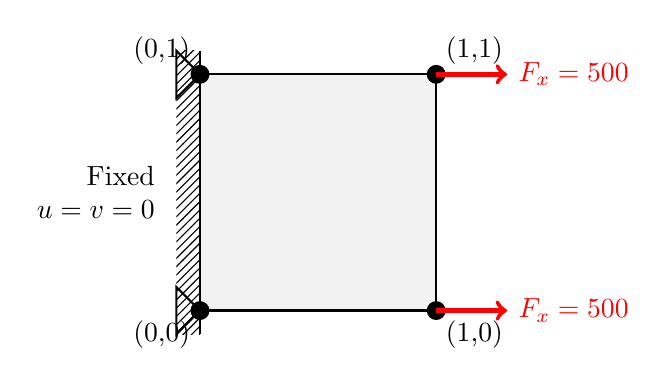
\begin{tikzpicture}[scale=3]
        % Define Coordinates
        \coordinate (N1) at (0,0);
        \coordinate (N2) at (1,0);
        \coordinate (N3) at (1,1);
        \coordinate (N4) at (0,1);

        % Draw Element
        \draw[thick, fill=gray!10] (N1) -- (N2) -- (N3) -- (N4) -- cycle;

        % Draw Nodes
        \foreach \pt in {N1,N2,N3,N4} \fill[black] (\pt) circle (0.04);

        % Node Labels
        \node[below left] at (N1) {(0,0)};
        \node[below right] at (N2) {(1,0)};
        \node[above right] at (N3) {(1,1)};
        \node[above left] at (N4) {(0,1)};

        % Boundary Condition (Fixed Wall on Left)
        \fill[pattern=north east lines] (-0.1,-0.1) rectangle (0,1.1);
        \draw[thick] (0,-0.1) -- (0,1.1);
        
        % BC Symbols (Triangles)
        \draw[thick] (N1) -- ++(-0.1,-0.1) -- ++(0,0.2) -- cycle;
        \draw[thick] (N4) -- ++(-0.1,-0.1) -- ++(0,0.2) -- cycle;
        \node[left, align=right] at (-0.15, 0.5) {Fixed\\$u=v=0$};

        % Load Arrows
        \draw[->, ultra thick, red] (N2) -- ++(0.3,0) node[right] {$F_x = 500$};
        \draw[->, ultra thick, red] (N3) -- ++(0.3,0) node[right] {$F_x = 500$};
        
        % Dimensions
        %\draw[<->] (0,-0.2) -- (1,-0.2) node[midway, below] {$L=1.0$};
        %\draw[<->] (1.5,0) -- (1.5,1) node[midway, right] {$H=1.0$};

    \end{tikzpicture}
    \caption{Single element test case with boundary conditions and loads.}
\end{figure}

\subsection*{Theoretical Solution}

The problem approximates a bar under axial tension. The theoretical stress and displacements are calculated using the basic mechanics of materials principles.

\subsubsection*{1. Axial Stress ($\sigma_{xx}$)}
\begin{equation}
    \sigma_{xx} = \frac{P}{A} = \frac{1000 }{1.0 \times 1.0}  = \mathbf{1000}
\end{equation}

\subsubsection*{2. Axial Displacement ($\delta_x$)}
The elongation of the element at $x=L$:
\begin{equation}
    \delta_x = \frac{P L}{A E} = \frac{1000 \times 1.0}{1.0 \times 30 \times 10^6} = \mathbf{3.333 \times 10^{-5} \text{ unit}}
\end{equation}

\subsubsection*{3. Lateral Displacement ($\delta_y$)}
Due to the Poisson effect, the material contracts in the transverse direction.
\begin{equation}
    \epsilon_{yy} = -\nu \epsilon_{xx} = -\nu \left( \frac{\sigma_{xx}}{E} \right) = -0.3 \left( \frac{1000}{30 \times 10^6} \right) = -1.0 \times 10^{-5}
\end{equation}
Total contraction:
\begin{equation}
    \delta_y = \epsilon_{yy} \times H = \mathbf{-1.0 \times 10^{-5} \text{ unit}}
\end{equation}

\textit{Note:} Since the left edge is fully constrained ($v=0$), the numerical FEA result for $\delta_y$ at the free end (Nodes 2 and 3) may vary slightly depending on whether the Poisson effect is constrained by the element formulation. However, but for a single element constant-stress patch, it typically matches the theoretical prediction.

\subsection*{Result from Code}
The results obtained from the MATLAB finite element code are presented below. The displacements are scaled by $1.0 \times 10^{-4}$ in.

\subsubsection*{1. Nodal Displacements}
\begin{center}
\begin{tabular}{|c|c|c|c|}
\hline
\textbf{Node} & \textbf{X } & \textbf{Y } & \textbf{Result ($u, v$)} \\ \hline
1 & 0 & 0 & $(0, 0)$ \\ \hline
2 & 1 & 0 & $(3.234 \times 10^{-5}, \phantom{-}0.669 \times 10^{-5})$ \\ \hline
3 & 1 & 1 & $(3.234 \times 10^{-5}, -0.669 \times 10^{-5})$ \\ \hline
4 & 0 & 1 & $(0, 0)$ \\ \hline
\end{tabular}
\end{center}

\textbf{Observation:} The computed axial displacement ($3.234 \times 10^{-5}$) is approximately $3\%$ times stiffer than the theoretical value ($3.333 \times 10^{-5}$). This is expected because the fully fixed boundary ($v=0$ at $x=0$) prevents the material from contracting naturally at the support, introducing artificial stiffness (Poisson locking effect).

\subsubsection*{2. Element Stresses (Gauss Points)}
\begin{center}
\begin{tabular}{|c|c|c|c|c|}
\hline
\textbf{GP} & \textbf{$\sigma_{xx}$ } & \textbf{$\sigma_{yy}$ (unit)} & \textbf{$\tau_{xy}$ (unit)} & \textbf{Von Mises (psi)} \\ \hline
1 & 1038.21 & 226.62 & 44.57 & 948.64 \\ \hline
2 & 961.79 & -28.09 & 44.57 & 979.19 \\ \hline
3 & 961.79 & -28.09 & -44.57 & 979.19 \\ \hline
4 & 1038.21 & 226.62 & -44.57 & 948.64 \\ \hline
\textbf{Avg} & \textbf{1000.0} & \textbf{99.2} & \textbf{0.0} & \textbf{-} \\ \hline
\end{tabular}
\end{center}

\textbf{Observation:}
\begin{itemize}
    \item \textbf{Axial Stress ($\sigma_{xx}$):} The average stress is exactly \textbf{1000 unit}, matching the theoretical prediction perfectly. The variation ($\pm 38$ unit) is due to the bending moment induced by the fixed support preventing lateral contraction.
    \item \textbf{Transverse Stress ($\sigma_{yy}$):} Significant stress ($\approx 226$ unit) appears at Gauss Points 1 and 4 (near the wall). This confirms that the fixed boundary ($v=0$) forces the material to generate internal stress to resist the Poisson contraction.
    \item \textbf{Conclusion:} The code is correctly solving the elasticity equations. The deviation from the simple $P/A$ theory is not a code error, but a consequence of the boundary condition ($u=v=0$) being more restrictive than the theoretical assumption (roller support).
\end{itemize}

\begin{figure}[t!]
    \centering
    \includegraphics[width=0.7\textwidth]{test1.png}
    \caption{Superimposed deformed and undeformed  shape (scale factor = 10000) of the element}
    \label{fig:your_label}
\end{figure}
\newpage
\section*{Test Case 2: Plate with a Central Circular Hole}

To verify the code's ability to handle irregular isoparametric elements, a stress concentration problem is analyzed. The problem consists of a rectangular plate with a central circular hole subjected to uniaxial tension.

\subsection*{Problem Definition}

\begin{itemize}
    \item \textbf{Global Geometry:} 
    \begin{itemize}
        \item Plate Width $w = 100$ 
        \item Hole Diameter $d = 10$  (Radius $R = 5$ )
        \item Thickness $t = 1.0$ 
        \item Geometric Ratio: $d/w = 10/100 = 0.1$
    \end{itemize}
    \item \textbf{Modeled Domain:} Due to symmetry, only one quarter of the plate is modeled ($50 \times 50$  region).
    \item \textbf{Material:} Steel ($E = 30 \times 10^6$ , $\nu = 0.3$).
    \item \textbf{Boundary Conditions (Symmetry):}
    \begin{itemize}
        \item Left Edge ($x=0$): $u = 0$
        \item Bottom Edge ($y=0$): $v = 0$
    \end{itemize}
    \item \textbf{Loading:} Uniform tensile force applied at the right edge.
    \begin{equation*}
        P_{total} = 50,000 \text{ unit (arbitrary load)}
    \end{equation*}
\end{itemize}

\subsection*{Theoretical Solution (Finite Width Correction)}

For a plate of finite width, the theoretical stress concentration factor $K_t$ is slightly lower than the infinite plate solution ($K_t=3.0$). Based on standard stress concentration charts (e.g., Shigley Fig A-15-1) for $d/w = 0.1$:
\begin{equation}
    K_t \approx 2.72
\end{equation}

\subsubsection*{1. Nominal Stress ($\sigma_0$)}
The nominal stress is calculated based on the \textbf{net cross-sectional area} at the hole (the smallest area):
\begin{equation}
    A_{net} = (w - d) \times t = (50 - 5) \times 1 = 45 \text{ unit}
\end{equation}
\begin{equation}
    \sigma_0 = \frac{P_{total}}{A_{net}} = \frac{50,000}{45} = \mathbf{1111.11 \text{ unit}}
\end{equation}

\subsubsection*{2. Theoretical Maximum Stress ($\sigma_{max}$)}
The maximum stress occurs at the top of the hole ($x=0, y=R$):
\begin{equation}
    \sigma_{max}^{theory} = K_t \times \sigma_0 = 2.72 \times 1111.11 = \mathbf{3022.2 \text{ unit}}
\end{equation}

\subsection*{Finite Element Model Setup}

The mesh is generated by mapping the circular boundary of the hole to the square outer boundary of the plate using isoparametric Q4 elements.

\begin{figure}[h]
    \centering
    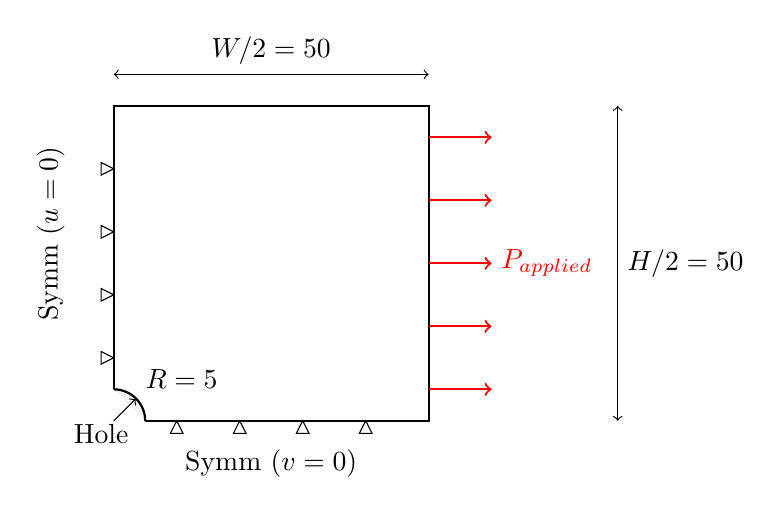
\begin{tikzpicture}[scale=0.08] % Scale down because dimensions are 50mm
        % Define Coordinates
        \coordinate (Center) at (0,0);
        \coordinate (TopLeft) at (0,50);
        \coordinate (TopRight) at (50,50);
        \coordinate (BottomRight) at (50,0);
        
        % Draw Outer Box
        \draw[thick] (0,5) -- (0,50) -- (50,50) -- (50,0) -- (5,0);
        
        % Draw Hole Arc (Radius 5)
        \draw[thick, fill=gray!10] (5,0) arc (0:90:5);
        \node at (-2,-2) {Hole};

        % Draw Symmetry BCs
        % Left Edge
        \foreach \y in {10,20,30,40} {
            \draw (0,\y) -- ++(-2,-1) -- ++(0,2) -- cycle; % Triangles
        }
        \node[left, rotate=90] at (-10,45) {Symm ($u=0$)};

        
        % Bottom Edge
        \foreach \x in {10,20,30,40} {
            \draw (\x,0) -- ++(-1,-2) -- ++(2,0) -- cycle; % Triangles
        }
        \node[below] at (25, -3) {Symm ($v=0$)};

        % Load Arrows (Right Edge)
        \foreach \y in {5,15,25,35,45} {
            \draw[->, thick, red] (50,\y) -- ++(10,0);
        }
        \node[right, red] at (60, 25) {$P_{applied}$};

        % Dimensions
        \draw[<->] (0,55) -- (50,55) node[midway, above] {$W/2 = 50$};
        \draw[<->] (80,0) -- (80,50) node[midway, right] {$H/2 = 50$};
        \draw[->] (0,0) -- (3.5,3.5) node[above right] {$R=5$};

    \end{tikzpicture}
    \caption{Quarter-symmetry finite element model showing boundary conditions.}
\end{figure}




\subsection*{Mesh}
The mesh is imported from an Abaqus file of a similar model and pasted into the code in the nodes and elements list of Main\_Project.m. 
\begin{figure}[t!]
    \centering
    \includegraphics[width=0.7\textwidth]{mesh2.png}
    \caption{Mesh Imported from Abaqus}
    \label{fig:mesh2}
\end{figure}
\newpage
\subsection*{Boundary Condition}

The $x$–displacement of all nodes on the left edge is zero. \\
The $y$–displacement of all nodes on the bottom edge is zero. \\
The load in the $x$–direction on all the right edge nodes is distributed as 
$50{,}000 = 1923 \times 26$. (Here, 26 is the number of nodes on the right edge) \\[6pt]

u(x=0, y) = 0, \qquad 
v(x, y=0) = 0, \qquad
$F_x$(x=L, y) = 1923.

\subsection*{Numerical Results}

The maximum stress occurs in the element directly above the hole ($90^\circ$ position). The stress results at the four integration points (Gauss Points) for this critical element are listed below:

\begin{center}
\begin{tabular}{|c|c|c|c|c|}
\hline
\textbf{GP} & \textbf{$\sigma_{xx}$ (MPa)} & \textbf{$\sigma_{yy}$ (MPa)} & \textbf{$\tau_{xy}$ (MPa)} & \textbf{Von Mises (MPa)} \\ \hline
1 & 2541.68 & 66.87 & -93.06 & 2514.08 \\ \hline
2 & 2545.37 & 62.14 & -17.99 & 2515.07 \\ \hline
\textbf{3} & \textbf{2951.84} & 184.20 & -23.82 & 2864.48 \\ \hline
4 & 2947.93 & 189.21 & -103.18 & 2863.61 \\ \hline
\end{tabular}
\end{center}

\subsubsection*{Analysis of Results}
\begin{itemize}
    \item \textbf{Peak Stress:} The maximum computed stress is $\sigma_{xx} = 2951.84$ MPa at Gauss Point 3.
    \item \textbf{Accuracy:} Comparing this to the theoretical value of $3022$ MPa:
    \begin{equation}
        \% \text{ Error} = \frac{|3022 - 2951.8|}{3022} \times 100 \approx \mathbf{2.3\%}
    \end{equation}
    \item \textbf{Variation within Element:} Gauss points 3 and 4 show significantly higher stresses than points 1 and 2. This is expected because points 3 and 4 are physically located closer to the inner radius ($r=R$), where the stress concentration is highest. Points 1 and 2 are further out radially, where the stress gradient drops steeply.
    \item \textbf{Conclusion:} The FEA code accurately captures the stress concentration with an error of less than 3\%, validating the implementation of the isoparametric Q4 element and the Jacobian mapping.
\end{itemize}
\begin{figure}[t!]
    \centering
    \includegraphics[width=0.7\textwidth]{deformed_mesh2.png}
    \caption{Superimposed deformed and undeformed  shape (scale factor = 10000) of the model}
    \label{fig:your_label}
\end{figure}

\subsection*{Acknowledgments}
I acknowledge the assistance of Gemini (Google) and ChatGPT (OpenAI) in the development and debugging of the finite element code and the preparation of this documentation.

\begin{thebibliography}{9}
\bibitem{shigley} 
Budynas, R. G., \& Nisbett, J. K. (2015). \textit{Shigley’s Mechanical Engineering Design} (10th ed.). New York, NY: McGraw-Hill Education.
\end{thebibliography}

\end{document}



